%!TEX root = ../stoeter_sourcecount.tex
\section{Evaluation Results}%
\label{sec:evaluation}
In this section we perform several experiments on the proposed CRNN model that has been selected in the previous section.
We assess the performance of this model by showing the results of three experiments that augment the test data by
choosing a different dataset, varying amplitude gain levels and introduce reverberation.
These results also include several baseline methods.
Furthermore we present the effect of training sample duration and compare the results from the DNN to human performance gathered in an listening experiment.

\subsection{Baselines}%
\label{ssec:baselines}
In order to make a meaningful comparison to the CRNN model we propose several baseline methods.
Since we are dealing with a novel task description, related speaker count estimation techniques like those introduced in Section~\ref{sec:introduction}, can hardly be used as baselines.
Specifically,~\cite{xu13} would not work on fully overlapped speech,~\cite{andrei15_interspeech} does not scale to the size of our dataset, since it requires to cross correlate the full database against another.
Finally,~\cite{sayoud10} proposes a feature but does not employ a fully automated system that can be used in a data-driven context.
We therefore decided to propose our own baseline methods.

\paragraph*{\textbf{VQ}}
This method uses a feature proposed by Sayoud~\cite{sayoud10} based on 7th MEL filter coefficient (\(\mbox{MFCC}_7\)) which was shown to encode sufficiently important speaker related information.
The temporal dimension of \(X\) is squashed down by subtracting the mean and standard deviation as \(X = \overline{\mbox{MFCC}_7} - STD(\mbox{MFCC}_7) \in \mathbb{R}^{1}\).
In~\cite{sayoud10} the mapping from \(X \Rightarrow \cardinality \) is done by manually thresholding \(X\).
To translate this into a data-driven approach, we employed a vector quantizer (using k-means) to get an optimal mapping with respect to the sum of squares criterion.
Further, as preprocessing, we added the same normalization as for our proposed CRNN which in turn decreases the performance of the method significantly as it is highly gain dependent.

\paragraph*{\textbf{SVM, SVR}}
We found that the information encoded in the 7th \(\mbox{MFCC}\) coefficient as used in the \textbf{VQ} baseline, may not be sufficient enough to  explain the high variability in our dataset.
This is especially important for larger speaker counts.
We therefore extended \textsc{VQ} by including all 20 MFCCs but using the same temporal dimensionality reduction, resulting in \(X = \overline{MFCC} - STD(MFCC) \in \mathbb{R}^{20}\).
To deal with significantly increased dimensionality of \(X\), we used a support vector machine (SVM) with a radial basis function (RBF) kernel.
Similarly to our proposed DNN based methods, we treat the output as either a classification problem or a regression problem through the use of support vector regression (SVR).

\subsection{Results on Gain Variations}%
\label{ssec:exp_random_gains}
% * Pick: STFT, Classification
% * 0db =1.0 gain randomly varied between 0.5 and 2.0
% * Performance drops slightly
%
% * --> CNN and CRNN, are most robust to gain variation
\begin{table*}[h]
\caption{Averaged MAE results of different methods on several datasets for \( k = [0 \ldots 10] \) with $0~\mbox{dB}$ SNR and Random gains (up to $\pm 3~\mbox{dB}$) SNR) as well as reverberation. Bold face indicates the best performing method.}
\begin{center}
\begin{tabular}{lcccccccc}
\toprule
Trained on & \multicolumn{7}{c}{\emph{LIBRI 0~dB SNR}} & \multicolumn{1}{c}{\emph{LIBRI-Reverb}} \\
\cmidrule(r){2-8} \cmidrule(r){9-9}
Test Set & \multicolumn{3}{c}{LIBRI} & \multicolumn{2}{c}{THCS10} & \multicolumn{2}{c}{TIMIT} & \multicolumn{1}{c}{LIBRI-Reverb} \\
\cmidrule(r){2-4} \cmidrule(r){5-6} \cmidrule(r){7-8} \cmidrule(r){9-9}
Variation &     – &     $\pm 3~\mbox{dB}$ SNR  & Reverb &  – &     $\pm 3~\mbox{dB}$ SNR  &     – &  $\pm 3~dB$ SNR & Reverb \\
\midrule
CRNN    &  $\mathbf{0.27 \pm{0.22}}$ & $\mathbf{0.43 \pm{0.39}}$ & $1.63 \pm{0.22}$ & $\mathbf{0.36 \pm{0.25}}$  & $\mathbf{0.50 \pm{0.46}}$ & $\mathbf{0.31 \pm{0.33}}$ & $\mathbf{0.52 \pm{0.52}}$  &  $\mathbf{0.48 \pm{0.22}}$\\
SVR     &  $0.58 \pm{0.27}$ & $0.61 \pm{0.31}$ & $\mathbf{0.76 \pm{0.35}}$ & $0.69 \pm{0.28}$ &  $0.73 \pm{0.32}$ & $0.70 \pm{0.45}$ & $0.62 \pm{0.36}$ & $0.71 \pm{0.35}$ \\
SVC     &  $0.63 \pm{0.39}$ & $0.66 \pm{0.37}$ & $0.85 \pm{0.51}$ & $0.77 \pm{0.37}$ &  $0.77 \pm{0.36}$ & $0.89 \pm{0.75}$ & $0.76 \pm{0.61}$ & $0.78 \pm{0.45}$ \\
VQ \cite{sayoud10} &  $2.41 \pm{1.08}$ & $2.41 \pm{1.06}$ & $2.41 \pm{1.08}$ & $2.98 \pm{1.62}$ &  $2.98 \pm{1.60}$ & $2.13 \pm{1.06}$ & $2.15 \pm{1.07}$ & $2.41 \pm{1.13}$ \\
MEAN    &  $2.73 \pm{1.63}$ & $2.73 \pm{1.63}$ & $2.73 \pm{1.63}$ & $2.73 \pm{1.64}$ &  $2.73 \pm{1.63}$ & $2.73 \pm{1.63}$ & $2.73 \pm{1.63}$ & $2.73 \pm{1.63}$ \\
\bottomrule
\end{tabular}
\end{center}
\label{tab:expgainreverb}
\end{table*}
In our parameter optimization in Section~\ref{sec:hyperparameters} we evaluated on mixtures of 0~dB SNR, so that all speakers are equalized to the same energy level.
In a more realistic scenario, speakers often differ in volume between utterances.
We simulate this by introducing gain factors between 0.5 and 2.0, randomly applied on the 0~dB SNR sources, hence resulting in $[-3~dB \ldots 3~dB]$ SNR.
We applied this variation only on the test data to evaluate how models generalize to this updated condition.
The results of this experiment are presented in Table~\ref{tab:expgainreverb}.
\textbf{MEAN} corresponds to the case when \(\cardinality = 5\) is predicted for all test samples.
Our results indicate that augmenting the mixture gains does have an impact on performance, for both, our proposed CRNN model as well as the baseline methods.
E.g.\ for the CRNN model the performance drops by 60\% from 0.27 MAE to 0.43 MAE on the \emph{LIBRI Speech} test set, which is still about 40 \% better than the second best performing method \emph{SVR} which drops from 0.58 MAE to 0.61 MAE.\@

\subsection{Results on Different Datasets}%
\label{ssec:r_datasets}
We also present results on two additional datasets.
Again, we only changed the test data; all networks were trained on \emph{LIBRI Speech}.
Compared to \emph{LIBRI Speech}, the \emph{TIMIT} database has an overall lower recording quality.
This is reflected by our results where the performance in MAE drops only slightly between these two datasets.
Interestingly, even when we look at the results of the Mandarin language \emph{THCS10} dataset, performance drops only slightly.
More precisely, for our proposed CRNN model, test performance on \emph{THCS10} is even better than on its own \emph{LIBRI} dataset with gain variations.
These results show that the trained model is speaker and language independent.

% * Pick best: CRNN, STFT, Classification
% * TIMIT (slight drop)
% * German Dataset (medium drop)
% * THCS Chinese (large drop)

\subsection{Effect of Reverberant Signals}%
\label{ssec:exp_reverb}
% * Pick best: CRNN, STFT, Classification
% * Generated simulated using @hab RIR Generator
% * test room: [3.5, 4.5, 2.5]
% * receiver position at [1, 1, 1]
% * generating 350 RIRs for each room: between 100ms and 500ms
% * generating 10 unique source positions for each room: min distance 0.1 to walls
% * --> Significant Performance Drop (diff 2.0 MAE)
% * Retrained using train room: [3, 4, 2] and valid room: [4, 5, 3]
% * Performance back to (0.6 MAE)
Different acoustical conditions such as increased reverberation time was shown~\cite{Pasha17_reverb} to have a large effect in speaker counting.
To analyze this effect, different acoustic conditions were simulated by generating the room impulse responses using the image method~\cite{Allen79, Habets16}.
For this experiment we set up an acoustical room with dimension ($3.5~\mbox{m} \times 4.5~\mbox{m} \times 2.5~\mbox{m}$)
The microphone was positioned at (1m, 1m, 1m).
For the mentioned room, 350 different reverberation times were selected uniformly sampled between 0.1 and 0.5 seconds.
For each of these reverberation times, we generated unique room impulse responses that correspond to individual source positions which have minimum distance $0.1~\mbox{m}$ to the walls and are otherwise positioned randomly on the (X, Y, 1m) plane.
Each speaker's signal was convolved with a randomly selected room impulse response before mixing.
Results, again, are shown in Table~\ref{tab:expgainreverb}.
For the first time we can see that the CRNN model significantly drops in performance from 0.27 MAE to 1.64 MAE, whereas the SVR and SVM baselines are only affected slightly.
This is expected as the baselines do not have access to the temporal context that the CRNN has.
More precisely, the baselines are using a temporal aggregation of all frames, whereas the CRNN is based on smaller (\(3 \times 3\)) convolutional filter operations that are able to capture the room acoustics as well.
If we assume that our trained deep learning model is fully speaker independent, a mixture of two utterances from the same speaker would get the same count estimate as two different speakers.
Hence, reverberation then leads to overestimation.
This effect can be seen in the results of the CRNN which overestimates even for \(k = 1\), hence increasing the MAE significantly.
\par
To further investigate whether the overestimation can be reduced via training with reverberant samples, we created a separate set of room impulse responses for the training data set with different room dimensions so that the model does not memorize to learn the acoustical conditions from the training data set.
From the results shown in the last column of Table~\ref{tab:expgainreverb} we can see that the retrained CRNN is able to outperform the baselines again.
Therefore, when retrained with reverberant samples, the proposed model is able to better discriminate between reverberant component of the same speaker and contributions from different speakers.
For robustness against different acoustic conditions, it is essential to include reverberant samples in the training dataset.

\subsection{Effect of Duration}%
\label{ssec:exp_duration}
% * Pick best: CRNN, STFT, Classification
% * (Re) Trained and evaluated on (1s...9s)
% * Longer context
% * Shorter context
In our scenario  the true number of speakers depends on the input duration \(D\), thus for longer segments it is likely that a source is active at least once, whereas for very short segments.
In our last experiment we therefore want to address the influence of the input duration length \(D\).
In a real world application this parameter would be chosen as small as a possible, because a longer input duration adds both algorithmic and computational delay to a real time system.
In a small experiment we took the proposed CRNN and retrained it using a different number of input frames ranging from 100 to 900 frames (corresponding to one to nine seconds of audio).
For each input duration we trained the CRNN with three different initial seeds.
Results are shown in Figure~\ref{fig:timesteps}.
It can be seen that five second duration is a good trade-off between performance and delay.
If latency is critical, keeping \(D\) above 2s is recommended for sufficient results.

\begin{figure}[h!]
    \centering
    \centering
    \begin{adjustbox}{width=0.8\columnwidth}
      % This file was created by matplotlib2tikz v0.6.13.
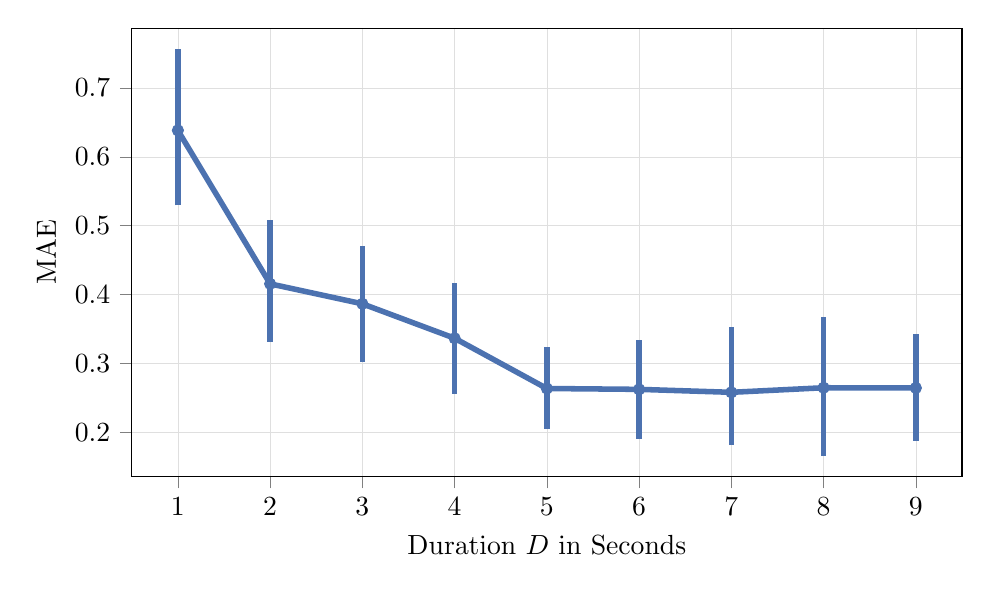
\begin{tikzpicture}

\definecolor{color1}{rgb}{0.298039215686275,0.447058823529412,0.690196078431373}
\definecolor{color0}{rgb}{0.917647058823529,0.917647058823529,0.949019607843137}

\begin{axis}[
xlabel={Duration \(D\) in Seconds},
ylabel={MAE},
xmin=-0.5, xmax=8.5,
ymin=0.135857456148673, ymax=0.786816272987562,
xtick={0,1,2,3,4,5,6,7,8},
xticklabels={1,2,3,4,5,6,7,8,9},
ytick={0.1,0.2,0.3,0.4,0.5,0.6,0.7,0.8},
yticklabels={0.0,0.2,0.3,0.4,0.5,0.6,0.7,},
tick align=outside,
tick pos=left,
xmajorgrids,
ymajorgrids,
width=\columnwidth,
height=0.6\columnwidth,
axis line style={black},
grid style={line width=.1pt, draw=gray!25},
major grid style={line width=.2pt,draw=gray!25},
]
\addplot [only marks, draw=color1, fill=color1, colormap/blackwhite]
table{%
x                      y
+0.000000000000000e+00 +6.385012990646495e-01
+1.000000000000000e+00 +4.156636288682126e-01
+2.000000000000000e+00 +3.866786050449682e-01
+3.000000000000000e+00 +3.366750172732503e-01
+4.000000000000000e+00 +2.637021331951673e-01
+5.000000000000000e+00 +2.624647418728959e-01
+6.000000000000000e+00 +2.581671791258833e-01
+7.000000000000000e+00 +2.647957418016120e-01
+8.000000000000000e+00 +2.645404355185759e-01
};
% \addplot[mark=*, fill=black, mark options={mark size=0.20pt}]
% coordinates {
%   (5, 0.26} node[pin={1, pin edge={thick}}:{Selected Duration}]{};
\addplot [line width=2.00pt, color1, forget plot]
table {%
0 0.638501299064649
1 0.415663628868213
2 0.386678605044968
3 0.33667501727325
4 0.263702133195167
5 0.262464741872896
6 0.258167179125883
7 0.264795741801612
8 0.264540435518576
};
\addplot [line width=2.00pt, color1, forget plot]
table {%
0 0.529501745070873
0 0.757227235858521
};
\addplot [line width=2.00pt, color1, forget plot]
table {%
1 0.331229177698919
1 0.50777318536896
};
\addplot [line width=2.00pt, color1, forget plot]
table {%
2 0.302866441412883
2 0.470527138303221
};
\addplot [line width=2.00pt, color1, forget plot]
table {%
3 0.256214672080081
3 0.416434186077932
};
\addplot [line width=2.00pt, color1, forget plot]
table {%
4 0.205581195002823
4 0.323809986137185
};
\addplot [line width=2.00pt, color1, forget plot]
table {%
5 0.190651073067454
5 0.334762156170043
};
\addplot [line width=2.00pt, color1, forget plot]
table {%
6 0.181574955025837
6 0.352612918248687
};
\addplot [line width=2.00pt, color1, forget plot]
table {%
7 0.165446493277713
7 0.367320912424733
};
\addplot [line width=2.00pt, color1, forget plot]
table {%
8 0.18797697232341
8 0.343365533924186
};
% \path [draw=black, fill opacity=0] (axis cs:500,0.135857456148673)
% --(axis cs:500,0.786816272987562);
%
% \path [draw=white, fill opacity=0] (axis cs:1,0.135857456148673)
% --(axis cs:1,0.786816272987562);
%
% \path [draw=white, fill opacity=0] (axis cs:-0.5,0)
% --(axis cs:8.5,0);
%
% \path [draw=white, fill opacity=0] (axis cs:-0.5,1)
% --(axis cs:8.5,1);

\end{axis}

\end{tikzpicture}

    \end{adjustbox}
    \caption{Evaluation of trained CRNN networks over different input duration length \(D\). Error bars show 95\% confidence intervals.}%
    \label{fig:timesteps}
 \end{figure}

\subsection{Listening Experiment}%
\label{ssec:listening_experiment}
% * Reference existing listening tests which report the same thing
% * Are we really doing it? We can decide on this once the first full draft is ready.
To compare the results of our trained CRNN on our synthesized dataset to human performance, we chose to reproduce the experiments made in~\cite{kawashima15, kashino96}.
Kawashima et al.\ found in extensive experiments using Japanese speech samples, that participants were able to correctly estimate up to three simultaneously active speakers without using any spatial cues.
We conducted our own study using the simulated data from the \emph{LIBRI Speech 0dB SNR} set mentioned earlier in Section~\ref{ssec:corpus}.
We therefore randomly selected 10 samples for each \(\cardinality \in [0, \ldots, 10]\), resulting in 100 mixtures of 5~seconds duration each.
The experiment was done using \emph{between-group design}, where one group (blind experiment) did not get any prior information about the maximum number of speakers in the test set (similar to~\cite{kawashima15}).
However, the maximum number of speakers was revealed to the other group (informed experiment), which is more related to our data-driven, classification based CRNN.
Further, none of the participants received any feedback about the error made during the trials.
Similarly to~\cite{kawashima15}, lab based experiments were conducted with ten participants for each group (\(n=20\)) using a custom designed web-based software.\footnote{The experiment is made available through the accompanying website.}
In all previous experiments, we used the mean absolute error metric which does not reveal over and underestimation errors.
We therefore decided to report the average response for each group of \(k\).
The results of our lab based experiments are shown in Figure~\ref{fig:experiment}.
The results for up to three speakers indicate that humans perform similarly (or better in terms of variance) compared to our proposed CRNN model.
Results of the blind experiment show that underestimation becomes apparent for \(k > 3\).
As a reference, we also included the average results from~\cite{kawashima15} (Experiment 1, 5~seconds durations) which shows similar results compared to our blind experiment.
For larger speaker counts, the gap between humans and algorithm is almost three speakers on average.
Interestingly, the results of the informed experiment reveal that this gap closes down to an average difference of one speaker.
Finally, we can report that the machine model reached superhuman performance. However, with extensive training, humans might be able to perform on par.
When we asked participants about the strategy they pursued, many reported that with more than three speakers it is not possible to identify (and count) the speakers but rather compare the \emph{density} of the speech to that of 1-3 speakers.
For higher speaker counts, participants reported that the integrated phoneme activity was a relevant cue, supporting our previously mentioned hypothesis.

\begin{figure}[ht!]
    \centering
    \begin{adjustbox}{width=0.7\columnwidth}
      % This file was created by matplotlib2tikz v0.6.13.
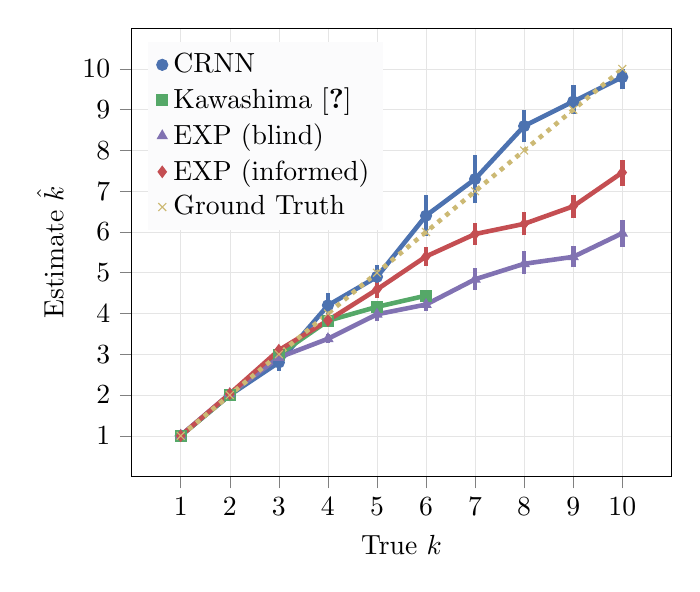
\begin{tikzpicture}

\definecolor{color1}{rgb}{0.298039215686275,0.447058823529412,0.690196078431373}
\definecolor{color0}{rgb}{0.917647058823529,0.917647058823529,0.949019607843137}
\definecolor{color4}{rgb}{0.768627450980392,0.305882352941176,0.32156862745098}
\definecolor{color2}{rgb}{0.333333333333333,0.658823529411765,0.407843137254902}
\definecolor{color5}{rgb}{0.8,0.725490196078431,0.454901960784314}
\definecolor{color3}{rgb}{0.505882352941176,0.447058823529412,0.698039215686274}

\begin{axis}[
xlabel={True \(k\)},
ylabel={Estimate \(\hat{k}\)},
xmin=-1, xmax=10,
ymin=0, ymax=11,
ytick={1,2,3,4,5,6,7,8,9,10},
xtick={0,1,2,3,4,5,6,7,8,9},
xticklabels={1,2,3,4,5,6,7,8,9,10},
tick align=outside,
tick pos=left,
ymajorgrids,
xmajorgrids,
grid style={line width=.1pt, draw=gray!20},
major grid style={line width=.2pt,draw=gray!20},
axis line style={black},
legend style={at={(0.03,0.97)}, anchor=north west, draw=none, fill=color0!20},
legend cell align={left},
legend entries={{CRNN},{Kawashima~\cite{kawashima15}}, {EXP (blind)}, {EXP (informed)},{Ground Truth}}
]
\addplot [only marks, draw=color1, fill=color1, colormap/blackwhite]
table{%
x                      y
+0.000000000000000e+00 +1.000000000000000e+00
+1.000000000000000e+00 +2.000000000000000e+00
+2.000000000000000e+00 +2.800000000000000e+00
+3.000000000000000e+00 +4.200000000000000e+00
+4.000000000000000e+00 +4.900000000000000e+00
+5.000000000000000e+00 +6.400000000000000e+00
+6.000000000000000e+00 +7.300000000000000e+00
+7.000000000000000e+00 +8.600000000000000e+00
+8.000000000000000e+00 +9.199999999999999e+00
+9.000000000000000e+00 +9.800000000000001e+00
};
\addplot [line width=1.66pt, color1, forget plot]
table {%
0 1
1 2
2 2.8
3 4.2
4 4.9
5 6.4
6 7.3
7 8.6
8 9.2
9 9.8
};
\addplot [line width=1.66pt, color1, forget plot]
table {%
0 1
0 1
};
\addplot [line width=1.66pt, color1, forget plot]
table {%
1 2
1 2
};
\addplot [line width=1.66pt, color1, forget plot]
table {%
2 2.5975
2 3
};
\addplot [line width=1.66pt, color1, forget plot]
table {%
3 4
3 4.5
};
\addplot [line width=1.66pt, color1, forget plot]
table {%
4 4.6
4 5.2
};
\addplot [line width=1.66pt, color1, forget plot]
table {%
5 5.9
5 6.9
};
\addplot [line width=1.66pt, color1, forget plot]
table {%
6 6.7
6 7.9
};
\addplot [line width=1.66pt, color1, forget plot]
table {%
7 8.2
7 9
};
\addplot [line width=1.66pt, color1, forget plot]
table {%
8 8.8975
8 9.6
};
\addplot [line width=1.66pt, color1, forget plot]
table {%
9 9.5
9 10
};
\addplot [only marks, mark size=2.0, mark=square*, draw=color2, fill=color2, colormap/blackwhite]
table{%
x                      y
+0.000000000000000e+00 +1.000000000000000e+00
+1.000000000000000e+00 +2.000000000000000e+00
+2.000000000000000e+00 +2.987442378071903e+00
+3.000000000000000e+00 +3.821715111593599e+00
+4.000000000000000e+00 +4.163430371330779e+00
+5.000000000000000e+00 +4.438511376242037e+00
};
\addplot [line width=1.66pt, color2, forget plot]
table {%
0 1
1 2
2 2.9874423780719
3 3.8217151115936
4 4.16343037133078
5 4.43851137624204
6 nan
7 nan
8 nan
9 nan
};
\addplot [line width=1.66pt, color2, forget plot]
table {%
0 nan
0 nan
};
\addplot [line width=1.66pt, color2, forget plot]
table {%
1 nan
1 nan
};
\addplot [line width=1.66pt, color2, forget plot]
table {%
2 nan
2 nan
};
\addplot [line width=1.66pt, color2, forget plot]
table {%
3 nan
3 nan
};
\addplot [line width=1.66pt, color2, forget plot]
table {%
4 nan
4 nan
};
\addplot [line width=1.66pt, color2, forget plot]
table {%
5 nan
5 nan
};
\addplot [line width=1.66pt, color2, forget plot]
table {%
6 nan
6 nan
};
\addplot [line width=1.66pt, color2, forget plot]
table {%
7 nan
7 nan
};
\addplot [line width=1.66pt, color2, forget plot]
table {%
8 nan
8 nan
};
\addplot [line width=1.66pt, color2, forget plot]
table {%
9 nan
9 nan
};

\addplot [only marks, mark size=2.0, mark=triangle*, draw=color3, fill=color3, colormap/blackwhite]
table{%
x                      y
+0.000000000000000e+00 +1.010000000000000e+00
+1.000000000000000e+00 +2.030000000000000e+00
+2.000000000000000e+00 +2.920000000000000e+00
+3.000000000000000e+00 +3.380000000000000e+00
+4.000000000000000e+00 +3.980000000000000e+00
+5.000000000000000e+00 +4.220000000000000e+00
+6.000000000000000e+00 +4.840000000000000e+00
+7.000000000000000e+00 +5.220000000000000e+00
+8.000000000000000e+00 +5.390000000000000e+00
+9.000000000000000e+00 +5.970000000000000e+00
};
\addplot [line width=1.66pt, color3, forget plot]
table {%
0 1.01
1 2.03
2 2.92
3 3.38
4 3.98
5 4.22
6 4.84
7 5.22
8 5.39
9 5.97
};
\addplot [line width=1.66pt, color3, forget plot]
table {%
0 1
0 1.03
};
\addplot [line width=1.66pt, color3, forget plot]
table {%
1 2
1 2.07
};
\addplot [line width=1.66pt, color3, forget plot]
table {%
2 2.78975
2 3.05
};
\addplot [line width=1.66pt, color3, forget plot]
table {%
3 3.27
3 3.5
};
\addplot [line width=1.66pt, color3, forget plot]
table {%
4 3.80975
4 4.16025
};
\addplot [line width=1.66pt, color3, forget plot]
table {%
5 4.06
5 4.4
};
\addplot [line width=1.66pt, color3, forget plot]
table {%
6 4.58
6 5.11
};
\addplot [line width=1.66pt, color3, forget plot]
table {%
7 4.97
7 5.53
};
\addplot [line width=1.66pt, color3, forget plot]
table {%
8 5.13
8 5.66
};
\addplot [line width=1.66pt, color3, forget plot]
table {%
9 5.64
9 6.29
};
\addplot [only marks, mark size=2.0, mark=diamond*, draw=color4, fill=color4, colormap/blackwhite]
table{%
x                      y
+0.000000000000000e+00 +1.000000000000000e+00
+1.000000000000000e+00 +2.030000000000000e+00
+2.000000000000000e+00 +3.100000000000000e+00
+3.000000000000000e+00 +3.830000000000000e+00
+4.000000000000000e+00 +4.590000000000000e+00
+5.000000000000000e+00 +5.400000000000000e+00
+6.000000000000000e+00 +5.950000000000000e+00
+7.000000000000000e+00 +6.200000000000000e+00
+8.000000000000000e+00 +6.630000000000000e+00
+9.000000000000000e+00 +7.460000000000000e+00
};
\addplot [line width=1.66pt, color4, forget plot]
table {%
0 1
1 2.03
2 3.1
3 3.83
4 4.59
5 5.4
6 5.95
7 6.2
8 6.63
9 7.46
};
\addplot [line width=1.66pt, color4, forget plot]
table {%
0 1
0 1
};
\addplot [line width=1.66pt, color4, forget plot]
table {%
1 1.97
1 2.1
};
\addplot [line width=1.66pt, color4, forget plot]
table {%
2 3
2 3.21
};
\addplot [line width=1.66pt, color4, forget plot]
table {%
3 3.67
3 3.98
};
\addplot [line width=1.66pt, color4, forget plot]
table {%
4 4.39
4 4.8
};
\addplot [line width=1.66pt, color4, forget plot]
table {%
5 5.16
5 5.64
};
\addplot [line width=1.66pt, color4, forget plot]
table {%
6 5.69
6 6.23
};
\addplot [line width=1.66pt, color4, forget plot]
table {%
7 5.91975
7 6.48
};
\addplot [line width=1.66pt, color4, forget plot]
table {%
8 6.34
8 6.92
};
\addplot [line width=1.66pt, color4, forget plot]
table {%
9 7.14
9 7.76025
};
\addplot [only marks, mark size=2.0, draw=color5, mark=x, fill=color5, colormap/blackwhite]
table{%
x                      y
+0.000000000000000e+00 +1.000000000000000e+00
+1.000000000000000e+00 +2.000000000000000e+00
+2.000000000000000e+00 +3.000000000000000e+00
+3.000000000000000e+00 +4.000000000000000e+00
+4.000000000000000e+00 +5.000000000000000e+00
+5.000000000000000e+00 +6.000000000000000e+00
+6.000000000000000e+00 +7.000000000000000e+00
+7.000000000000000e+00 +8.000000000000000e+00
+8.000000000000000e+00 +9.000000000000000e+00
+9.000000000000000e+00 +1.000000000000000e+01
};
\addplot [line width=1.66pt, color5, dotted, forget plot]
table {%
0 1
1 2
2 3
3 4
4 5
5 6
6 7
7 8
8 9
9 10
};
\addplot [line width=1.66pt, color5, forget plot]
table {%
0 nan
0 nan
};
\addplot [line width=1.66pt, color5, forget plot]
table {%
1 nan
1 nan
};
\addplot [line width=1.66pt, color5, forget plot]
table {%
2 nan
2 nan
};
\addplot [line width=1.66pt, color5, forget plot]
table {%
3 nan
3 nan
};
\addplot [line width=1.66pt, color5, forget plot]
table {%
4 nan
4 nan
};
\addplot [line width=1.66pt, color5, forget plot]
table {%
5 nan
5 nan
};
\addplot [line width=1.66pt, color5, forget plot]
table {%
6 nan
6 nan
};
\addplot [line width=1.66pt, color5, forget plot]
table {%
7 nan
7 nan
};
\addplot [line width=1.66pt, color5, forget plot]
table {%
8 nan
8 nan
};
\addplot [line width=1.66pt, color5, forget plot]
table {%
9 nan
9 nan
};
\end{axis}

\end{tikzpicture}

    \end{adjustbox}
    \caption{Average responses from humans (\emph{EXP} and \emph{Kawashima}
~\cite{kawashima15}) compared to our proposed CRNN. Error bars show 95\% confidence intervals.}%
    \label{fig:experiment}
 \end{figure}
